\nocite{srssbrs} % Sequential/Session-based Recommendations: Challenges, Approaches, Applications and Opportunities

\section*{Introdução}

Esse projeto tem como propósito a produção de um material didático
sobre sistemas de recomendação sequenciais.
O objetivo é apresentar uma visão geral sobre o assunto, enquanto
apresentamos uma abordagem de implementação de sistemas de recomendação
sequenciais baseada em  redes neurais de atenção.

\section*{Metodologia}

Para esse projeto, iremos utilizar o algoritmo de recomendação
\textit{Self-Attentive Sequential Recommendation (SASRec)} \cite{sasrec}.
Esse algoritmo proposto por Wang-Cheng Kang e Julian McAuley em 2018
consiste em uma rede neural de atenção que é treinada para prever o
próximo item a ser recomendado em uma recomendação sequencial.

Além disso, iremos utilizar o dataset de reproduções de músicas
do site \url{last.fm} disponível em \citeurl{lastfm_dataset}
\cite{lastfm_dataset} por \citeauthor{lastfm_book} \cite{lastfm_book}.

Esse dataset de 2010 apresenta o histórico de reprodução de músicas
de uma amostra de 1.000 usuários. Pela natureza do \url{last.fm},
cada usuário tem em média aproximadamente 20 mil reproduções de músicas,
resultando em um total de aproximadamente 19 milhões de reproduções
de músicas no dataset.

Produzimos um notebook disponível em \url{https://github.com/LiviaLelis/recsys-tp-seq},
junto ao material textual do projeto e instruções de uso. O notebook em
si apresenta constítui boa parte do material e explicações.

Além disso, foi produzida uma vídeo aula explicativa sobre sistemas de
% TODO: Adicionar link
recomendação sequencial disponível em \url{https://youtu.be/3-4-5-6},
para dar uma breve introdução ao assunto e apresentar as implementações
feitas neste projeto.

Esse material então foi enviado para algumas pessoal que atuam com 
conhecimento técnico na área de computação junto a um formulário de
avaliação de projeto para medir a qualidade do trabalho produzido.

\section*{Implementação}

\subsection*{Dataset}

Para o dataset, fizemos algumas modificações para adequar-se
as necessidades do algoritmo. Primeiramente, fizemos um
mapeamento dos UUIDs (universally unique identifier) para inteiros
sequenciais a partir do 1, já que necessitamos de representações
numéricas para os algoritmos.

Além disso, devido à natureza do \url{last.fm}, cada usuário tem
um volume extenso de reproduções de músicas. Entendemos que esse
histórico extenso pode ser dívido em "sessões de reprodução", 
isto é, um conjunto de reproduções de músicas que ocorrem de 
maneira quase contínua no tempo. Portanto, para cada usuário,
construímos um conjunto de sessões, tomando como critério para
uma sessão a reprodução de músicas que ocorrem em um intervalo
máximo de 30 minutos entre duas reproduções consecutivas. Acreditamos
que essa abordagem de tratamento de dados seja mais adequada para
o problema, reduzindo o tamanho das sequências e mantendo-as mais
coerentes, já que as preferências musicais de um usuário pode variar
entre sessões e com o tempo, entretanto não conseguimos medir se
essa assunção é verdadeira.

\subsection*{Modelo de Atenção}

Como mencionado anteriormente, para o modelo de atenção, utilizamos
o \citename{sasrec}. Esse modelo é baseado em uma rede neural de
atenção.

Esse modelo lançado em 2018 foi um dos primeiros algoritmos de
recomendação sequencial baseado nas redes neurais de atenção, sendo
lançado bem próximo ao artigo \citetitle{attetionisallyouneed} \cite{attetionisallyouneed}
trazendo essa ideia para o campo de sistemas de recomendação sequenciais.

\begin{figure}[H]
    \centering
    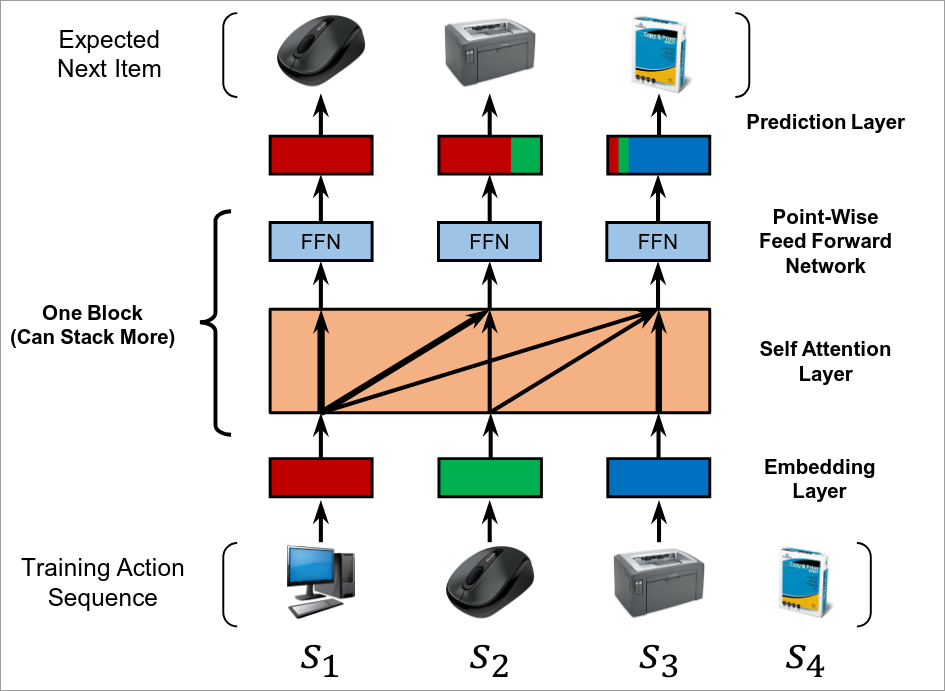
\includegraphics[width=0.6\textwidth]{../assets/sasrec-diagram.png}
    \caption{Diagrama da arquitetura do modelo SASRec \cite{sasrec}}
    \label{fig:sasrec-diagram}
\end{figure}

Como podemos ver na figura \ref{fig:sasrec-diagram}, o modelo SASRec
é bastante semelhante a outros modelos de atenção.

Nossa implementação é baseada em uma adaptação \cite{seanswyi} em
PyTorch do modelo dos autores originais implementado em TensorFlow.
Nessa adaptação, não fizemos mudanças diretas na arquitetura do
modelo, mas apenas algumas adaptações de código para melhorar a
legibilidade e marginalmente o desempenho. Além disso, desviamos
da implementação original nos parâmetros escolhidos, otimizador
e outras configurações.

A versão final do modelo foi treinada com uma amostra aleatória
de 100 mil sessões para reduzir o tempo de treinamento ao custo
de uma perda potencialmente pequena de qualidade. Além disso,
para a divisão dos dados, fizemos uma divisão de treino, teste
e validação pela estratégia sugerida pelos autores de truncamento
das sessões, isto é, todas as divisões contêm todas as sessões,
sendo que na divisão de treino é descartada os dois últimos itens
da sessão, na de validação o último item da sessão e na de teste
é mantida a sessão inteira. Como nosso volume de dados era
suficientemente grande, acreditamos que poderíamos obter resultados
mais realistas se seguíssemos uma divisão por meio das sessões em
si ao invés deste truncamento.

Além disso, para melhorar a performance do modelo, mantívemos a
estratégia original de construção de amostras negativas, isto é,
geramos para cada item um conjunto de itens negativos para que o
treinamento seja mais eficiente, realizando uma classificação
binária de se o item é positivo ou negativo.

A função de perda utilizada para avaliar o modelo foi a 
\textit{Binary Cross Entropy with Logits}, que é uma função de perda
para classificação binária. Além disso fizemos uso do algoritmo
de otimização AdamW \cite{adamw} com o parâmetro de learning rate
controlado por um \textit{scheduler OneCycleLR} \cite{onecyclelr}.

Mais informações sobre os parâmetros escolhidos podem ser vistas
no repositório do projeto disponível em \url{https://github.com/LiviaLelis/recsys-tp-seq}.

% Os parâmetros escolhidos para o modelo são:
%
% \begin{itemize}
%     \item \textit{batch size}: 512
%     \item \textit{max sequence length}: 50
%     \item \textit{dropout probability}: 0.4
%     \item \textit{hidden dimension}: 64
%     \item \textit{attention heads}: 2
%     \item \textit{epochs}: 500
%     \item \textit{AdamW beta 1}: 0.9
%     \item \textit{AdamW beta 2}: 0.999
%     \item \textit{AdamW epsilon}: 1e-8
%     \item \textit{AdamW weight decay}: 0.01
%     \item \textit{OneCycleLR warmup}: 5\%
%     \item \textit{OneCycleLR max learning rate}: 0.04
%     \item \textit{OneCycleLR annealing}: linear
% \end{itemize}

Após 3 hora e 50 minutos de treinamento em uma RTX 3080TI, obtivemos
os seguintes resultados:

\begin{itemize}
  \item \textbf{NDCG@10 Validação}: 0.681
  \item \textbf{HIT@10 Validação}: 0.777
  \item \textbf{NDCG@10 Teste}: 0.653
  \item \textbf{HIT@10 Teste}: 0.749
\end{itemize}

O modelo nesse período parece não ter convergido, provavelmente
conseguindo atingir resultados ainda melhores com um tempo de
treinamento maior.

\begin{figure}[H]
    \centering
    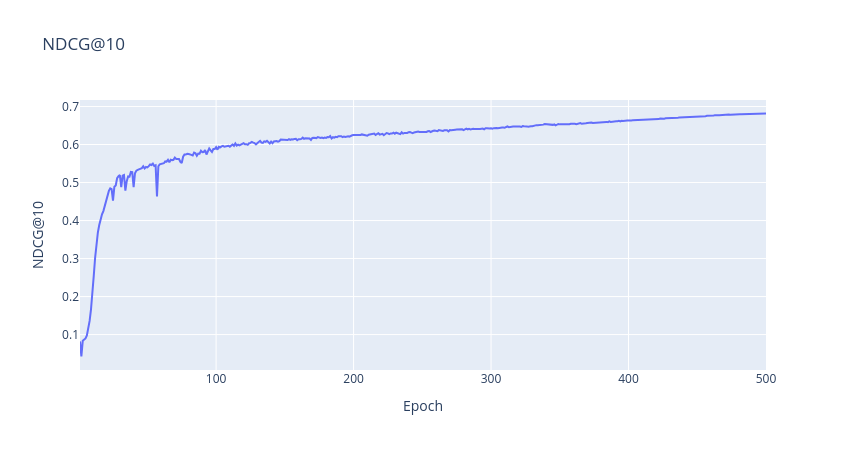
\includegraphics[width=0.6\textwidth]{../assets/validation-ndcg.png}
    \caption{Gráfico da métrica NDCG@10 na validação durante treinamento}
\end{figure}

\begin{figure}[H]
  \centering
  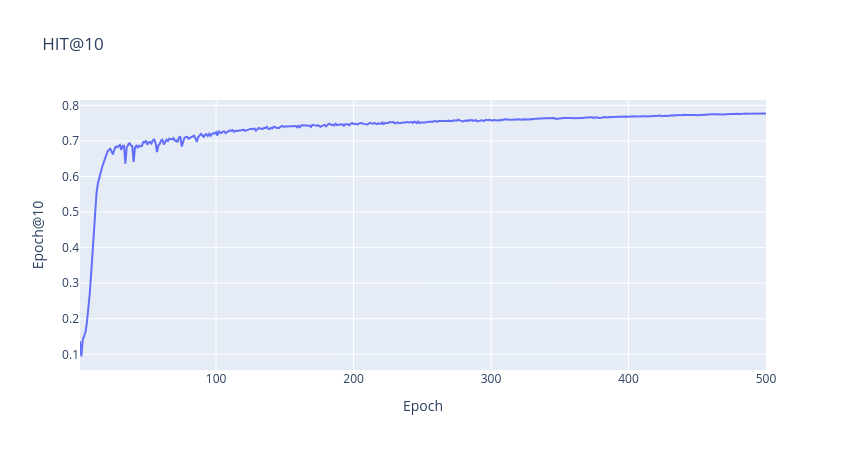
\includegraphics[width=0.6\textwidth]{../assets/validation-hit.png}
  \caption{Gráfico da métrica HIT@10 na validação durante treinamento}
\end{figure}

Os resultados obtidos são bastante interessantes, estando comparáveis
aos resultados obtidos para outros conjuntos de dados no artigo original
\cite{srssbrs}.

\section*{Avaliação do material}

TODO :)
